\documentclass[12pt]{article}
\usepackage{helvet}
\usepackage{amsfonts,amssymb,amsmath,color,graphicx,alltt}

%\textwidth = 7.5in
%\baselineskip = .1667in
%\oddsidemargin = -0.5in
%\textheight = 9.5in
%\headheight = 0in
%\headsep = 0in
%\topmargin = 0in

\textwidth = 6.5in
\baselineskip = .1667in
\oddsidemargin = 0.0in
\textheight = 8.5in
\headheight = 0in
\headsep = 0in
\topmargin = 0in

\begin{document}

%\title{reconstruct2contourtiler: converting from Reconstruct3D output
%to contour\_tiler input}

\title{Contour filtering for smoother surface meshes}

\author{Justin Kinney}

\maketitle

\section{Introduction}

Neuropil reconstruction from EM images begins with a process called
segmentation. The goal of segmentation is to divide each EM image into
regions corresponding to different anatomical structures. For example the
software program Reconstruct3D allows the user to outline regions with
contours consisting of a set of discrete points defined by mouse clicks.
After segmentation the regions are annotated by assigning names to the
contours so that sets of contours belonging to the same object can be
collected together. A surface mesh of the object can then be generated
by passing the collection of all contours belonging to a particular
object to a program such as VolumeRover that skins the contours by
connecting adjacent contours with triangular polygons. The quality of
the surface meshes is strongly influenced by the quality of the contour
points. Erratic contour profiles with points located in haphazard fashion
will contribute to noisy, uneven surfaces. In contrast contours will
smooth profiles and uniformly spaced points will support the generation
of smooth surfaces. This document describes the objectives, design,
and operation of a c++ software program for filtering contour points
before tiling to promote better output surface meshes.

%Intend to independently assess validity of objectives, merits of design,
%and success of implementation. Were any important objectives omitted?
%Is there a faster, more efficient, or more robust design that meets
%these objectives? Does the application interface need tweaking?

\section{Objectives}

Reconstructing a chunk of rat CA1 neuropil has
demonstrated a correlation between the quality of contour points passed
to VolumeRover and the quality of surface meshes generated as output.
A quality surface mesh is smooth with equilateral triangular
polygons. We have found that (1) smoothing the contours and (2) controlling the
distance between contour points to be near uniform before the tiling
operation greatly increases the output mesh quality. Here we describe
in more detail the motivation behind these two principal objectives of
the software. To illustrate the need for contour filtering we will be
referring to the trace in Figure \ref{fig:raw_and_sample_overlay_em}
arbitrarily chosen as representative of input contour data to the tiling
software.

\begin{figure}[htb]
  \begin{center}
    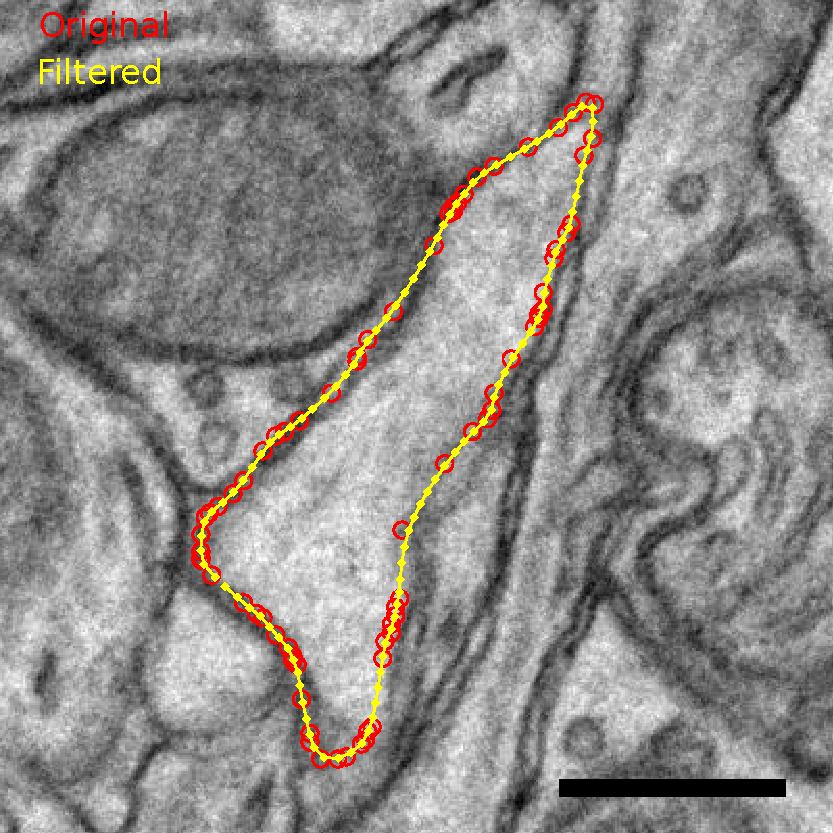
\includegraphics[width=10cm]{figures/raw_and_sample_overlay_em.pdf}
    \caption{\textbf{Profile smoothness and interval uniformity are
    improved.} Our example data set is one of nine contours belonging
    to a large apical dendrite (d000) on section 99 in Kristen Harris'
    rat CA1 data set labeled R34CA1-B. Note that the contour points
    (red) as originally traced are slightly rough in profile (but not
    by much in this example) and have a high variance of intersample
    point distance. By fitting cubic splines to the original points
    and resampling, the filtered contour points (yellow) are smoother
    with a dramatic improvement in interval uniformity. Note that
    the splines do not necessarily interpolate the original points, a
    point discussed in more detail later. Scale bar is 250 nanometers.}
    \label{fig:raw_and_sample_overlay_em}
  \end{center}
\end{figure}

\subsection{Contour profile smoothing}

To obtain smooth surface meshes the profiles of the contours are 
smoothed before tiling. So instead of using the original contour
points directly, splines are fit to the input points and then sampled.
Sets of four sequential contour points are used as control points for
nonrational, uniform cubic B-splines. In general the number of splines
used to describe a contour is equal to the number of original contour
points. Rather than constrain the splines to precisely interpolate
the contour points, the splines represent a weighted function of the
control points and consequently simply pass near the control points
(Figure \ref{fig:smoothing}). Consequently, the splines tend to smoothly
transition from one contour point to the next.

\begin{figure}[htb]
  \begin{center}
    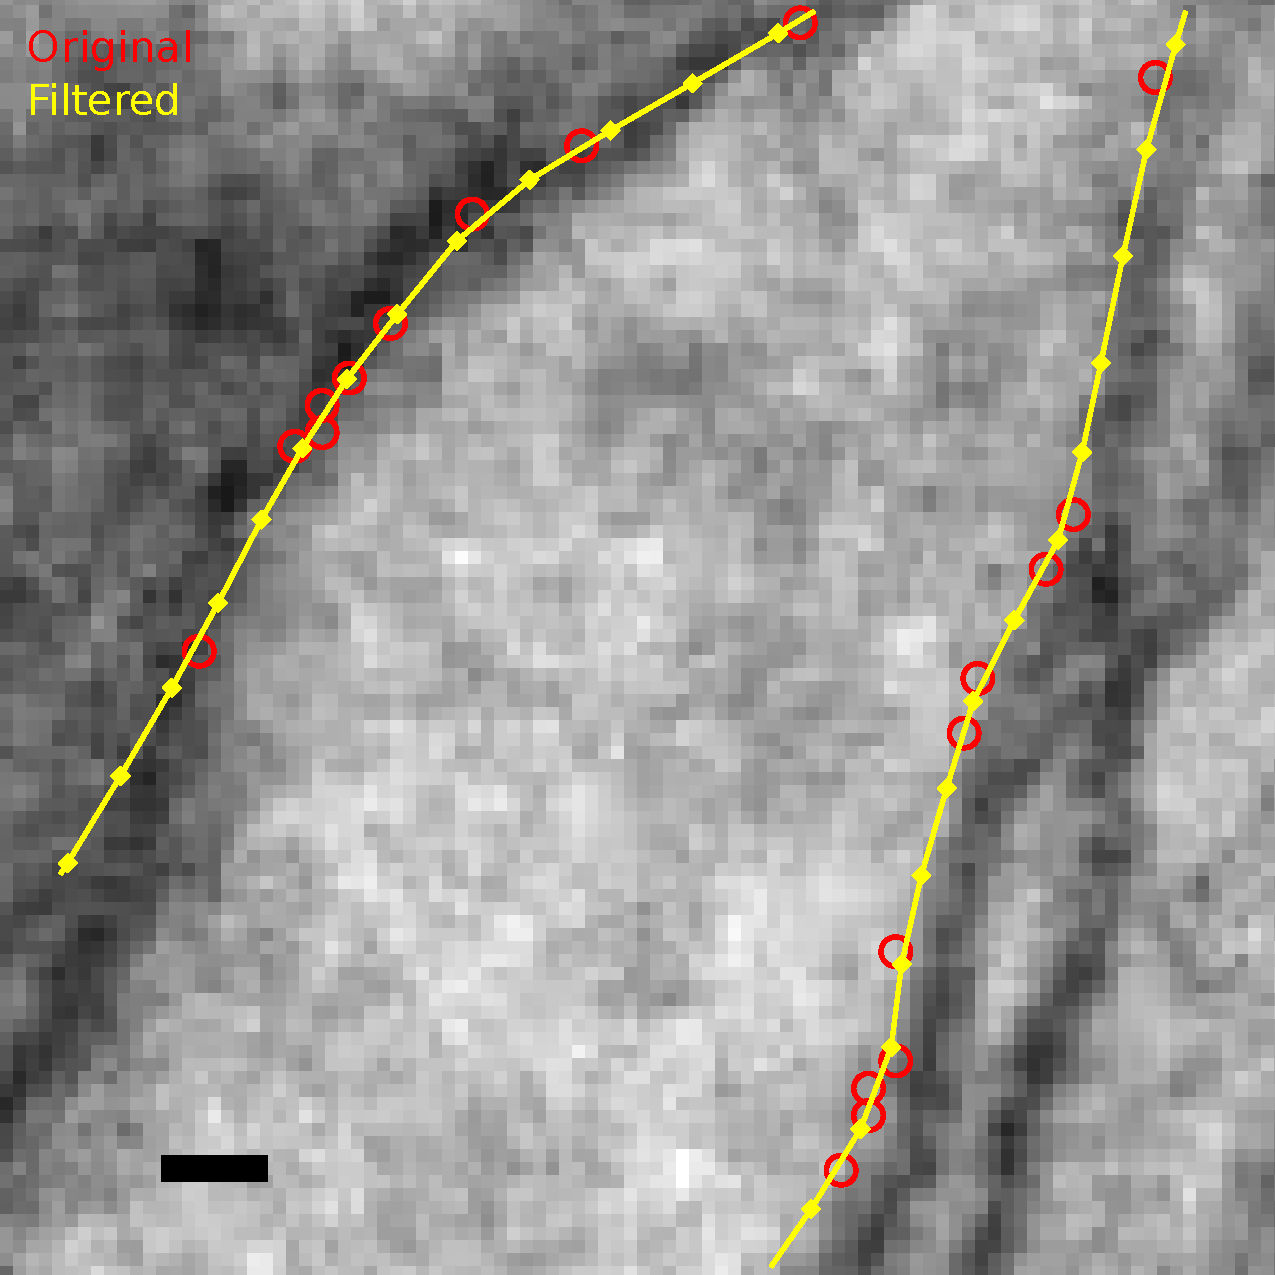
\includegraphics[width=10cm]{figures/smoothing.pdf}
    \caption{\textbf{Splines smoothly transition from one contour
    to the next.} B-splines are fit to the original contour points
    (red) and resampled yielding a smoother profile (yellow) than the
    original contour. In essence, the original contour is being run
    through a spatial low-pass filter. Scale bar is 20 nanometers.}
    \label{fig:smoothing}
  \end{center}
\end{figure}

Because the splines do not pass through the original contour points, the
spline samples are likely to be displaced some nonzero distance away from
the original contour. In fact, this deviation distance can be quite large.
For example, the maximum deviation observed in the entire CA1 contour data
set is larger than 40 nanometers. Consequently, provision is made in
the software to constrain the deviation between spline samples and the
original contour to be less than a user-specified deviation threshold
(Figure \ref{fig:deviation_control}).

\begin{figure}[htb]
  \begin{center}
    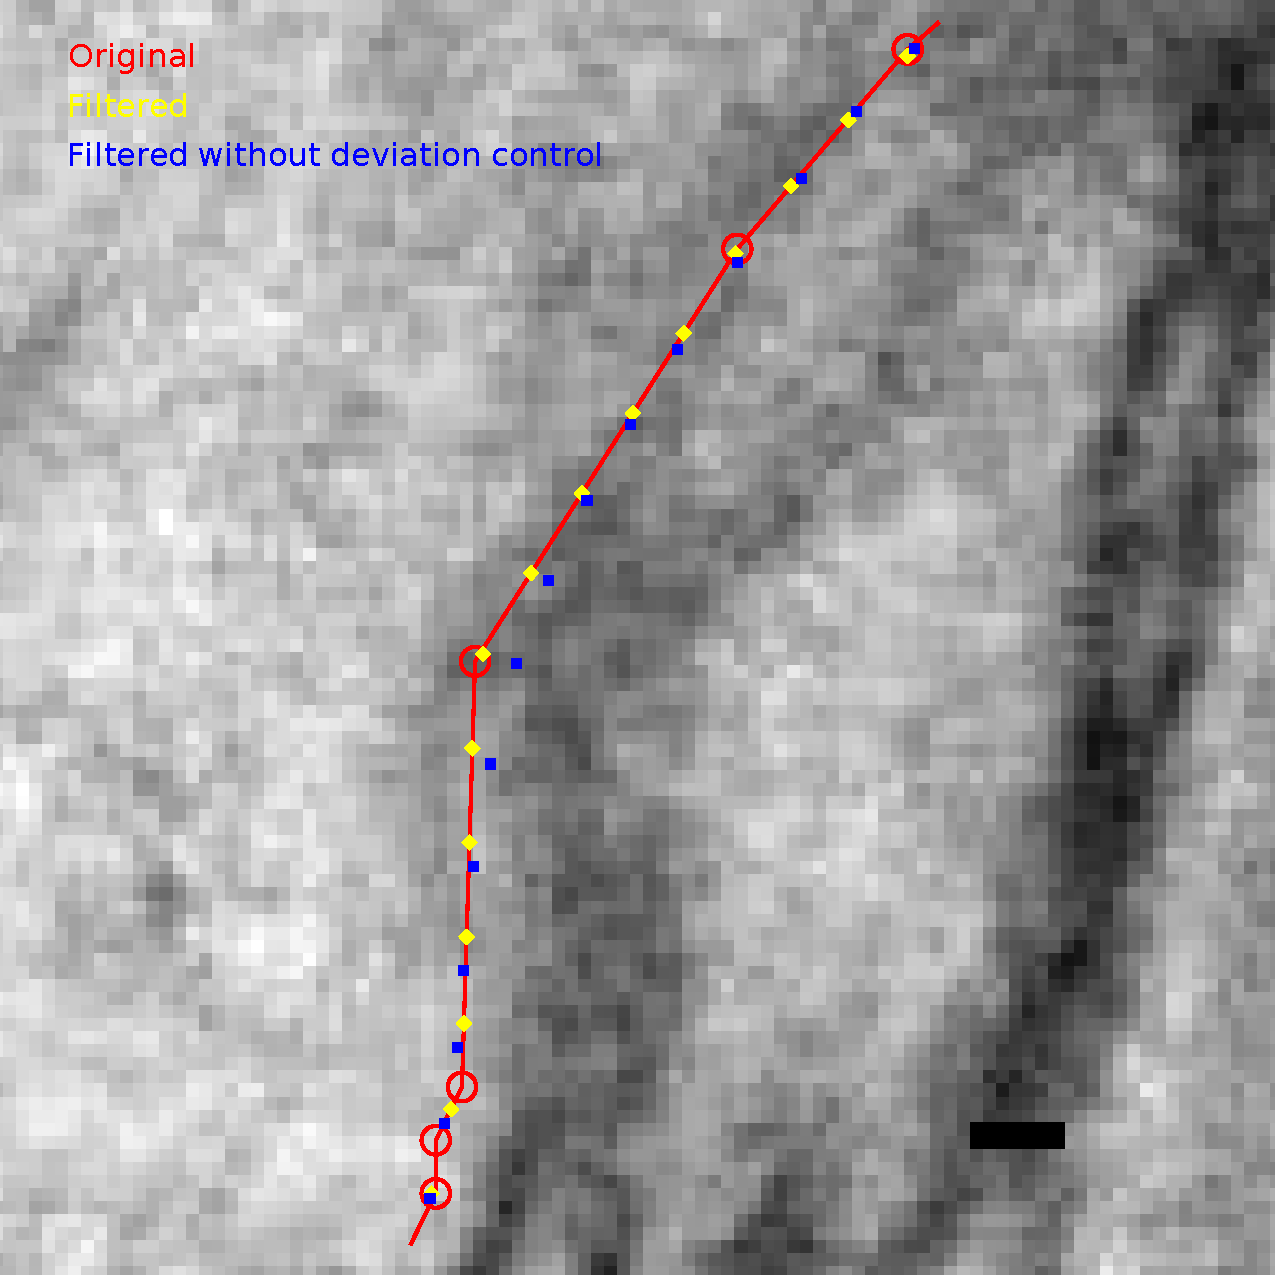
\includegraphics[width=10cm]{figures/deviation_control.pdf}
    \caption{\textbf{Deviation between original contour and spline
    samples is constrained to be less than user-specified threshold.}
    Without deviation control the spline samples (blue) deviate from
    the original contour (red) by more than 6.5 nanometers (center red
    circle). However, imposing a maximum allowed deviation distance of 5
    nanometers reduces the maximum deviation to less than one nanometer
    (yellow). Scale bar is 20 nanometers.} \label{fig:deviation_control}
  \end{center}
\end{figure}

\subsection{Contour point interval uniformity}

As important as contour smoothness for generating smooth surface meshes
(if not more so) is the uniformity of the distance between contour
points. The surface meshing process can be described as a search for
the most parsimonious tiling that connects all the contour points on
adjacent sections. As a result large differences in the distributions
of contour points from one section to the next are not handled
gracefully. Additionally for a given section thickness both very small
and very large sampling intervals lead to undesirable high aspect ratio
polygons. In contrast contours with near uniform intersample spacing
are more easily tiled and lead to higher quality meshes based on our
experience with the CA1 reconstruction. If the sample intervals are
comparable to the section thickness, the output surface polygons are
near equilateral and the surface is relatively more smooth. Because the
distance between samples is so important to the generation of smooth
surface meshes, the sample interval is controlled by the software
(Figure \ref{fig:sample_interval_concentrated}).

\begin{figure}[htb]
  \begin{center}
    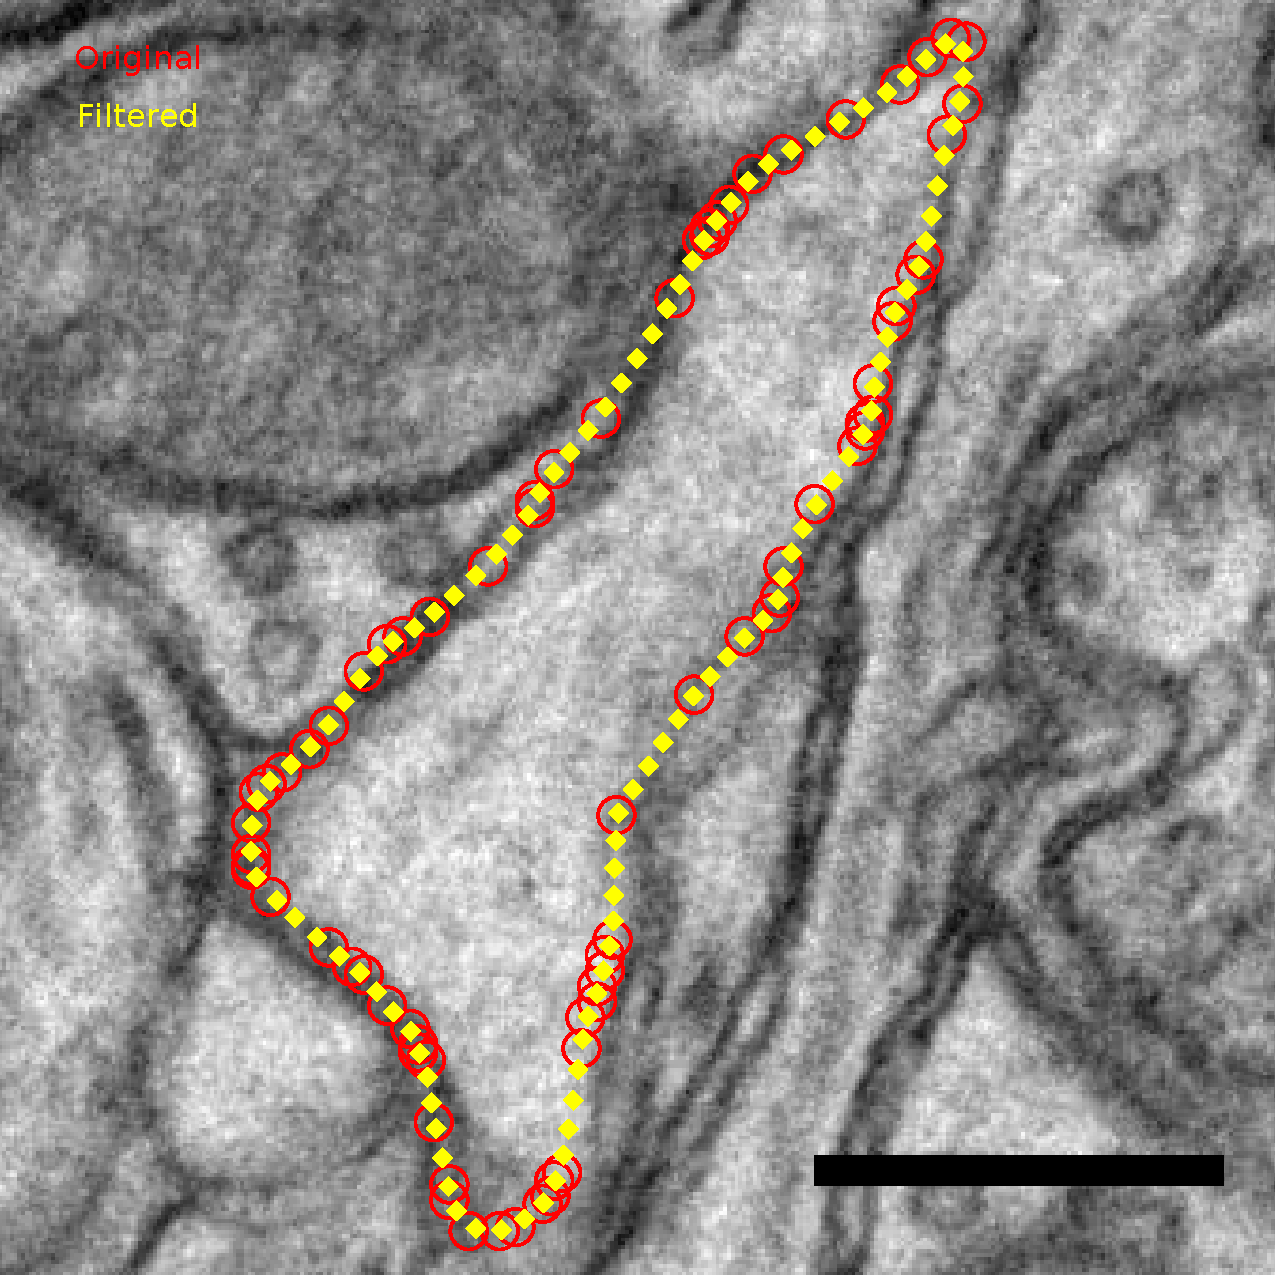
\includegraphics[width=10cm]{figures/sample_interval_concentrated.pdf}
    \caption{\textbf{Mesh smoothness is improved by controlling sample
    intervals.} The filtered points (yellow) correct three shortcomings
    of the original contour points (red). (1) The minimum sample interval
    was increased from 3 to 12 nanometers, thereby improving the aspect
    ratio of the thinnest polygons formed from the 50 nanometer section
    thickness. (2) The maximum sample interval was reduced from 90 to 20
    nanometers also improving the aspect ratio of the thickest polygons
    formed from the 50 nanometer section thickness. (3) The variance
    of the sample interval was reduced by two orders of magnitude which
    will promote smooth meshing with contours on adjacent sections. Scale
    bar is 250 nanometers.} \label{fig:sample_interval_concentrated}
  \end{center}
\end{figure}

We decided to explore two methods of controlling the sample intervals.
First, we implemented by far the simplest approach which is to use
uniform sample intervals. Second, we investigated an algorithm to place
more points at contour regions of high curvature and less points at
relatively straight contour regions. The rationale was that this method
would increase the information of each point to either better represent
the contour for a fixed number of points or represent a given contour
equally well with less points. Both methods are available in the software.

\subsection{Error detection}

The CA1 data set is contained in 101 input files defining 1640 different
objects described by 29952 individual contours with a total of 1521831
points. As if that were not already an incredible amount of data, future
reconstructions will contain orders of magnitude more. Because data
sets this massive will certainly contain errors, the software needs to
detect and handle a variety of errors in the contour data. For example,
the CA1 data set presents missing contours, duplicate points, contours
with less than three points, and contour names with characters prohibited
in file names. These anomalies and others like them are correctly
identified and dealt with appropriately.

\section{Design}

Piecewise-continuous cubic B-splines were chosen as the spline type for
this application since the splines have sufficient degrees of freedom to
represent the contour profile. Additionally, B-splines have the desirable
property that at the join point the splines are continuous in position,
slope, and curvature \cite{cgpp-2ed-1995}. Finally, B-splines do not
necessarily interpolate their control points which is exactly what we
had in mind. The fact that B-splines are a weighted function of their
control points and merely pass near them confers a degree of smoothness
to the splines that we wish to leverage here.

We specifically chose to use uniform, nonrational B-splines for several
reasons. First, the blending functions are the same for each spline
segment which makes computation of spline points very fast. (There is
no single set of blending functions for nonuniform B-splines, but there
may be a work around by restricting the path parameter to the range 0 to
1.) Second, the spline can be pulled toward a control point by duplicating
the control point once and even interpolate the point by copying again to
get a triple control point. In this application the contour points are the
control points, and it made sense to us to use them to control the shape
of the splines (rather than knots as is done with nonuniform B-splines).

Because the sample intervals are so important for the generation of
smooth meshes, we allow the user to specify a minimum and maximum sample
interval size. For example, the default maximum sample interval size is
set equal to the section thickness, and the minimum sample interval is
set to one-fifth of the maximum sample interval. These two values are
not used to enforce a strict sample interval policy; instead they are
used to guide the sampling of the splines in a more flexible way.
Specifically, the number of sample points per contour is constrained to be
greater than the contour length divided by he maximum sample interval
and less than the contour length divided by the minimum sample interval.
If the sample intervals are near uniform then each interval is likely
to fall within the range specified by the minimum and maximum values.

As mentioned above the software is designed to control sample intervals
by two different methods: uniform sample intervals and curvature-dependent
sampling. In the latter method the idea is to more densely sample splines
where the radius of curvature is small and sparsely sample where the
contour profile is more straight. We envision that the location of each
sample point is determined by opposing forces. One force concentrates
samples at regions of high curvature while an opposing force tries to
spread out the samples for uniform sample intervals. Since the curvature
of a cubic can be calculated exactly and the distance between samples
is also readily computable, we chose to cast the task of sample point
placement as an energy minimization problem and use simulated annealing
to find a local solution \cite{sim_anneal}. Briefly, simulated annealing
begins with a system at high "temperature" (i.e. randomized) and
randomly explores the local state space of the system always accepting
transitions that lower the energy of the system but also allowing with
some probability changes that raise the energy of the system. Thereby,
the system can escape local minima in search for the global minimum. As
the algorithm proceeds the "temperature" of the system is lowered by
reducing the probability of acceptance for moves that raise the system
energy, ultimately converging on a greedy algorithm. Theoretically, if the
temperature is lowered slow enough the system will find the global minimum.

The resulting placement of samples after simulated annealing depends
on the relative strength of the two opposing forces of curvature and
sample proximity. By heavily weighting the proximity energy the algorithm
returns samples more uniformly spaced irrespective of the curvature of
the contour profile. In the limit of zero curvature energy, uniform
sample intervals will be produced. Because the number of samples was
chosen based on the minimum and maximum sample intervals provided
by the user, then the uniform sample intervals will conform to these
constraints. On the other hand by heavily weighting the curvature energy
we retrieve samples densely concentrated in regions with low radius of
curvature at the expense of high sample interval variance. In the limit
of zero proximity energy then the distribution of sample intervals will
be multimodal with several clusters at large intervals and a cluster at
interval size of near zero. Because this scenario violates the minimum
and maximum sample interval constraints provided by the user, for the
curvature-dependent sampling method the balance of forces was carefully
tuned by trial and error. For most of the contours in the CA1 data set
the difference is small between the two sampling methods based on visual
inspection (Figure \ref{fig:uniform_vs_curvature_dependent}).

\begin{figure}[htb]
  \begin{center}
    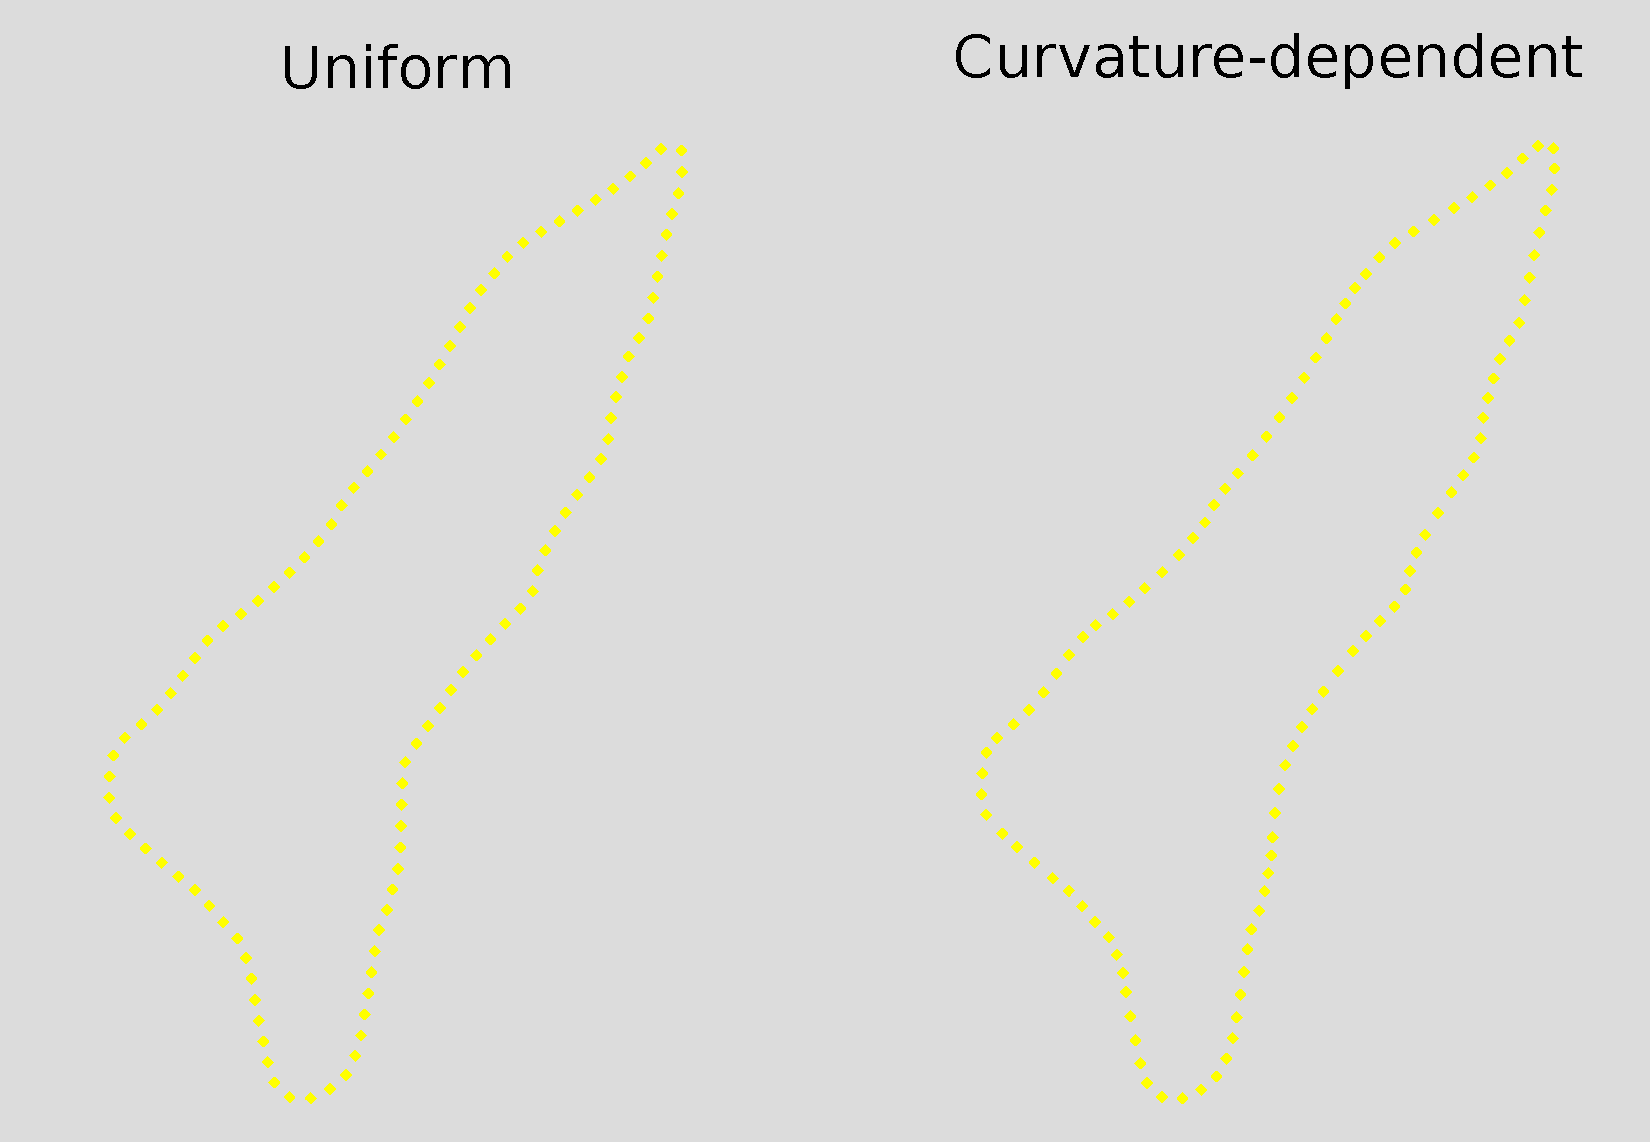
\includegraphics[width=10cm]{figures/uniform_vs_curvature_dependent.pdf}
    \caption{\textbf{Small difference between curvature-dependent and
    uniform sampling.} In this example the minimum sample interval was
    set to one-fifth of the maximum sample interval. Satisfying these
    constraints placed an upper bound on the relative weight of the
    curvature force with respect to proximity force. Consequently, the
    sampling patterns of the two methods are only slightly different.}
    \label{fig:uniform_vs_curvature_dependent}
  \end{center}
\end{figure}

The following sample interval statistics for the uniform and curvature-dependent
sampling methods quantify the difference between the samples shown in
Figure \ref{fig:uniform_vs_curvature_dependent}.

\begin{alltt}
\tiny
\input{histogram_uniform_samples.txt}
\end{alltt}

\begin{alltt}
\tiny
\input{histogram_concentrated_samples.txt}
\end{alltt}

\section{Operation}

The software has been tested in three basic modes of operation controlled
via command line switches. In the simplest usage the user requests
to get the original contour points back as output. In this mode the
software will process all contours found in files matching the given
name and section numbers in specified directory. The user has the option
of including command line directives to ignore scratch work contours,
especially exceptionally large contours. For instance, in the CA1 data
set a contour named domain1 was found on all sections and measured over
4000 microns in size. The user may wish to run in this mode to simply
get statistics on the sample interval of the original contour points.
Alternatively, future advances in automatic tracing algorithms will
deliver high quality contours that need no further processing.

In the second mode of operation the software linearly interpolates
the original contour points by constraining the sample points
to lie along straight lines between the original contour points. 
We chose to implement the linearity constraint by duplicating each
original contour point twice as control points. In this way the cubic
splines reduce to straight lines. While this approach is computationally
more expensive than alternatives, the process flow inside the code was
somewhat elegantly preserved. Because all straight lines have the same
curvature, uniform sample intervals are the only outcome.

In the third mode of operation the software fits cubic splines to the
contour points and samples the splines to generate new contour points.
Because each spline is a weighted sum of four different control points,
the splines does interpolate the contour points but instead pass near.
By changing the relative strength of the curvature force and proximity
force, the splines sample intervals can be uniform or concentrated at
contour regions of high curvature.

\section{TODO}

Perhaps the most important aspect of contour filtering that has not
been addressed here or in the software concerns the coordination
of contour points on adjacent sections. As discussed earlier
the smoothness of the output surface meshes is strongly affected by
gradients in the sample density on contours from adjacent sections.
Large changes in the sample density degrade the quality of the resulting
surface mesh.

Another topic of discussion is to decide whether to keep simulated
annealing. It is expensive and uniform sampling may be sufficient. As the
discussion above implies simulated annealing is used even when uniform
sampling is requested. The simulated annealing could almost certainly
be accelerated with a little work, but abandoning the annealing would
be faster still.

\section{Help Information}

\begin{alltt}
\tiny
\input{help_info.txt}
\end{alltt}

\bibliography{references.bib}{}
\bibliographystyle{plain}

\end{document}
